\documentclass[11pt]{article}
\usepackage[utf8]{inputenc}
\usepackage[english]{babel}
\usepackage{bilal2vec}

\title{SE 380 — HW 2}
\author{Bilal Khan\\
\href{mailto:bilal2vec@gmail.com}{bilal2vec@gmail.com}}
\date{\today}

\begin{document}

\maketitle

\tableofcontents

\section{1}

Consider the following model of a DC motor:

\[ G(s) = \dfrac{Y(s)}{U(s)} = \dfrac{K_m}{s(R_a (Js + b) + K_b K_m)} \]

where the value of all parameters is positive, the input $u(t) = \mathcal{L}^{-1}(U(s))$ is the voltage supplied to the motor, and the output $y(t) = \mathcal{L}^{-1}(Y(s))$ is the angle of the motor axle. Assume a unit step input voltage is supplied. 

\subsection{(a)} Find the transfer function betwen the angular speed - time derivative of the angle - and the input voltage.

\[ \omega(t) = y^\prime(t) \]
\[  G_\omega(s) = s G(s) = \dfrac{K_m}{R_a (Js + b) + K_b K_m} \]

\subsection{(b)} Find the steady-state angular speed of the motor axle

\begin{align*}
  \lim_{t \xrightarrow{} \infty} \omega(t) &= \lim_{s \xrightarrow{} 0} s G_\omega(s) U(s) \\
  &= \lim_{s \xrightarrow{} 0} s \dfrac{K_m}{R_a (Js + b) + K_b K_m} \dfrac{1}{s} \\
  &= \lim_{s \xrightarrow{} 0} \dfrac{K_m}{R_a (Js + b) + K_b K_m} = \dfrac{K_m}{R_a b + K_b K_m} \\
\end{align*}

\subsection{(c)} How long does the motor take to reach 99\% of its steady-state speed?

\begin{align*}
  G_\omega(s) &= \dfrac{K_m}{R_a (Js + b) + K_b K_m} \\
  &= \dfrac{K_m}{(R_a J) s + (R_a b + K_b K_m)} \\
  &= \dfrac{\frac{K_m}{R_a b + K_b K_m}}{\frac{R_a J}{R_a b + K_b K_m} s + 1} \\
\end{align*}

$\tau = \dfrac{R_a J}{R_a b + K_b K_m}$, we have that settling time @ 99\% is approximately $5 \tau = 5 \dfrac{R_a J}{R_a b + K_b K_m}$.

\section{2} 

Consider the following feedback control system.

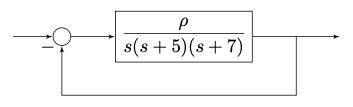
\includegraphics[width=200pt]{a3_q2.png}

Find the values of $\rho$ for which the closed-loop system is stable.

$L(s) = \dfrac{\rho}{s(s + 5)(s + 7)}$. We need to check if the poles of $1 + L(s)$ are in the left half of the plane.

\begin{align*}
  0 &= 1 + L(s) = 1 + \dfrac{\rho}{s(s^2 + 12s + 35)} \\
  &= 1 + \dfrac{\rho}{s^3 + 12s^2 + 35s} \\
  0 &= s^3 + 12s + 35s + \rho \\
\end{align*}

None of the given coefficients are negative, so we don't know if it is Hurwitz or not, all we can know is that for the system to be stable, $\rho > 0$.

\begin{table}[h]
  \centering
  \begin{tabular}{|c|c|c|}
  \hline
  $s^3$ & 1 & 35 \\
  $s^2$ & 12 & $\rho$ \\
  $s^1$ & $\frac{\rho}{12} - 35$ & 0 \\
  $s^0$ & $\rho$ & 0 \\
  \hline
  \end{tabular}
\end{table}

For all elements in the first column to be positive $\rho > 0$ and $\frac{\rho}{12} - 35 > 0$.

\begin{align*}
  \frac{\rho}{12} - 35 &> 0 \\
  \frac{\rho}{12} &> 35 \\
  \rho &> 420 \\
\end{align*}

The system is stable for $\rho > 420$.

\section{3}

Consider the following feedback control system.

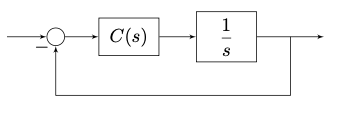
\includegraphics[width=200pt]{a3_q3.png}

Design a proportional controller a controller iwth transfer function $C(s) = K$ for some $K \in \mathbb{R}$ so that the closed-loop system satisfies the following specifications: It is stable, the steady state gain is $1$, and the settling time is less than $100ms$.

$L(s) = \dfrac{K}{s}$

$T(s) = \dfrac{L(s)}{1 + L(s)} = \dfrac{\frac{K}{s}}{1 + \frac{K}{s}} = \dfrac{K}{s + K}$

For the system to be stable, its poles are negative and so $K > 0$.

The steady-state gain is given by $\lim_{s \xrightarrow{} 0} s T(s) U(s) = \lim_{s \xrightarrow{} 0} \dfrac{K}{s + K} = \dfrac{K}{K} = 1$. So the steady-state gain is $1$. 

The settling time to 99\% is given by $5 \tau = 5 \dfrac{1}{K} < 0.1$. so $K > 50$.

This means that $C(s) = K$ for any $K > 50$

\end{document}
